\documentclass{article}
\usepackage[a4paper,margin=1in]{geometry}
\usepackage[utf8]{inputenc}
\usepackage[russian]{babel}
\usepackage{graphicx}
\graphicspath{ {./images/} }
\title{\Large Brick game: tetris. Документация}
\author{SIONAPAE}
\date{05.10.24}

\begin{document}
\maketitle

\begin{figure}[h]
\end{figure}
\section{Описание проекта}
Реализация игры «Тетрис» на языке программирования С с использованием структурного подхода.

\section{Требования}
Для запуска программы требуются:
\begin{itemize}
    \item Компилятор GCC или любой другой поддерживающий C++
    \item GNU Make для сборки программы
    \item библиотека check.h, ncurses.h
\end{itemize}

\section{Как собрать и запустить игру}
\begin{enumerate}
    \item Выполните команду `make all` для сборки программы.
    \item Запустите игру командой make run.
    \begin{itemize}
        \item all  
        \item install — компиляция исходного файла tetris
        \item run — запуск игры 
        \item uninstall — удаление tetris 
        \item clean — очистка файлов сборки
        \item dvi — документация проекта
        \item dist — архивирование 
        \item test — запуск тестов 
        \item gcov\_report — формирование html-отчета с информацией о покрытии функций тестами
    \end{itemize}
\end{enumerate}

\section{Управление}
Игрок использует клавиши на клавиатуре, имитирующие физические кнопки на реальной консоли, для управления падающими фигурками:
\begin{itemize}
    \item Клавиша D — Стрелка влево — перемещение фигуры влево.
    \item Клавиша A — Стрелка вправо — перемещение фигуры вправо.
    \item Клавиша F — Стрелка вниз — падение фигуры.
    \item Клавиша S — ускорение падения фигуры.
    \item Клавиша W — Стрелка вверх — поворот фигуры.
    \item Клавиша P/SPACE — пауза.
    \item Клавиша N/ENTER — старт новой игры или продолжение.
    \item Клавиша q/ESCAPE — завершение текущей игры, выход из игры.
\end{itemize}

\section{Архитектура программы}
Конечный автомат для конкретной реализации игры Тетрис.

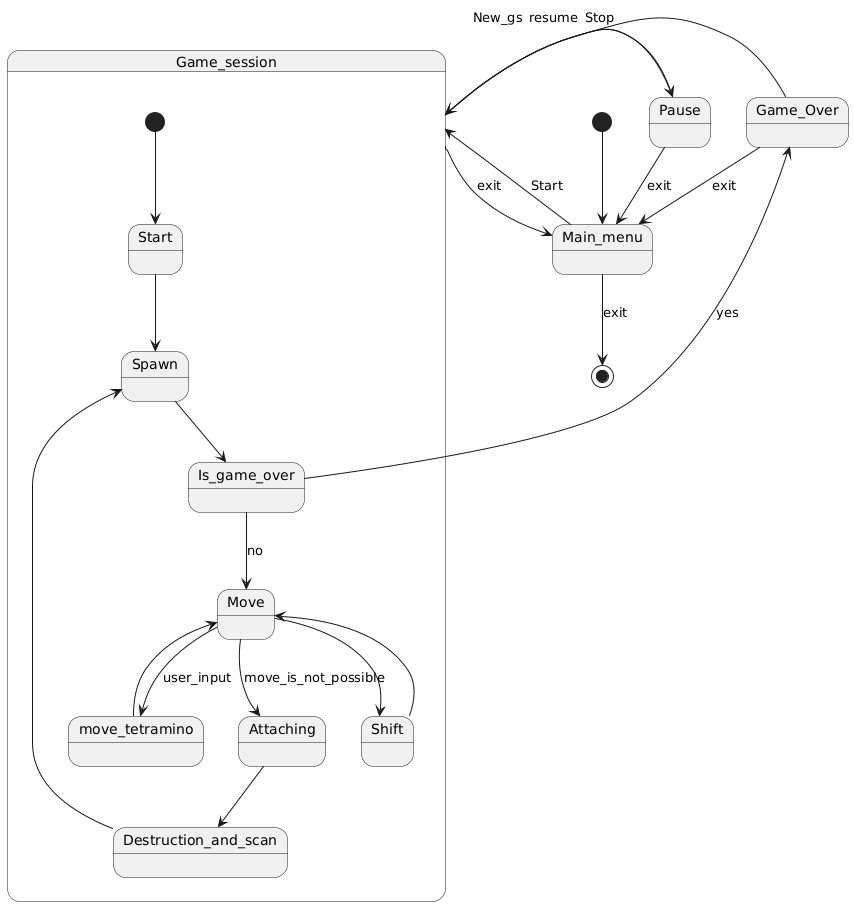
\includegraphics[width=10cm, height=10cm]{images/FSM.png}

\noindent Программа построена вокруг конечного автомата (Finite State Machine, FSM), который управляет логикой игры. Функция \texttt{main()} настраивает окружение, запускает игровой цикл через \texttt{game\_loop()} и обрабатывает завершение игры.

Весь код организован следующим образом:

\subsection{Функция \texttt{main()}: Точка входа}

Эта функция инициализирует окружение игры, запускает основной игровой цикл и завершает работу игры при выходе.

\begin{itemize}
    \item \textbf{Инициализация генератора случайных чисел:}
    \begin{verbatim}
    srand(time(0));
    get_random();
    \end{verbatim}
    Здесь инициализируется генератор случайных чисел для генерации случайных фигур Тетромино.
    
    \item \textbf{Инициализация игровых объектов:}
    \begin{verbatim}
    Game_Objects_t* params = get_instanse();
    *params = init_empty_game_objects();
    \end{verbatim}
    Объект \texttt{params} содержит информацию о текущем состоянии игры: текущее состояние, действия пользователя, игровые объекты и т.д.

    \item \textbf{Инициализация ncurses и запуск цикла игры:}
    \begin{verbatim}
    #ifndef debug_bro
    init_bro_ncurses(&params->views);
    game_loop();
    terminate_ncurses_bro(&params->views);
    #else
    game_loop();
    #endif
    \end{verbatim}
    В зависимости от режима компиляции, игра либо использует библиотеку ncurses для работы с консольным интерфейсом, либо запускается в режиме отладки без ncurses.
\end{itemize}

\subsection{Функция \texttt{game\_loop()}: Основной игровой цикл}

Цикл \texttt{game\_loop()} выполняется до тех пор, пока игра активна. Он обрабатывает все основные состояния игры и пользовательские действия.

\begin{itemize}
    \item \textbf{Инициализация состояния игры:}
    \begin{verbatim}
    State prev = START;
    \end{verbatim}
    Переменная \texttt{prev} хранит предыдущее состояние игры для возврата из паузы или других состояний.

    \item \textbf{Главный цикл игры:}
    \begin{verbatim}
    while (params->game_is_running) {
        draw_static(params);
        main_game_fsm(params);
        game_session(params, &prev);
    }
    \end{verbatim}
    Основной цикл игры продолжает выполняться до тех пор, пока \texttt{game\_is\_running == true}. Внутри цикла обрабатываются состояния игры и действия пользователя.
\end{itemize}

\subsection{Функция \texttt{game\_session()}: Управление игровой сессией}

Функция \texttt{game\_session()} управляет непосредственно игровым процессом (например, движением Тетромино, отсчетом времени и обработкой паузы).

\begin{itemize}
    \item \textbf{Инициализация игровой сессии:}
    \begin{verbatim}
    if (params->state == START) {
        session_is_running = true;
        params->state = *prev;
    }
    \end{verbatim}
    Если игра начинает с состояния \texttt{START}, то восстанавливается предыдущее состояние игры, и начинается новая игровая сессия.
    
    \item \textbf{Цикл игровой сессии:}
    \begin{verbatim}
    while (params->state != PAUSE && params->state != GAME_OVER && params->state != MAIN_MENU) {
        fsm_game_session(params);
        key = getch();
        userInput(getSignal(key), session_is_running);
        countTime(params);
    }
    \end{verbatim}
    Цикл продолжается до тех пор, пока игра не завершена (GAME\_OVER) или не поставлена на паузу. Внутри цикла обрабатываются пользовательские действия (движение, пауза, завершение игры) и обновляется состояние игрового мира.
    
    \item \textbf{Запись рекордов:}
    \begin{verbatim}
    if (params->gameInfo.score > params->gameInfo.high_score)
        write_high_score(params->gameInfo.score);
    \end{verbatim}
    Если игрок набрал новый рекордный счет, он записывается.
\end{itemize}

\section{Используемые технологии и библиотеки}

\begin{itemize}
    \item \textbf{Компилятор и версия:} Рекомендуемая версия — GCC 9.3
    \item \textbf{Внешние библиотеки:}
    \begin{itemize}
        \item \texttt{ncurses.h} — библиотека для работы с консольным интерфейсом, которая предоставляет функции для работы с текстовым терминалом, обработки ввода и вывода.
    \end{itemize}
\end{itemize}

\end{document}

